% Figure 3: C1 trajectory through the design space.
%   Past   — C1_old: Groth16 + per-circuit MPC starting point.
%   Present — C1 ★: PLONK + KZG + EF SRS reuse (the analyzed config).
%   Future — C7 ★★: Stellar + Plonky3 + FRI, host-blocked PQ destination.
%   Branch — C6 ★★: StarkNet + STARK, ready PQ destination, anchor change.
\begin{figure}[t]
  \centering
  \resizebox{\columnwidth}{!}{%
  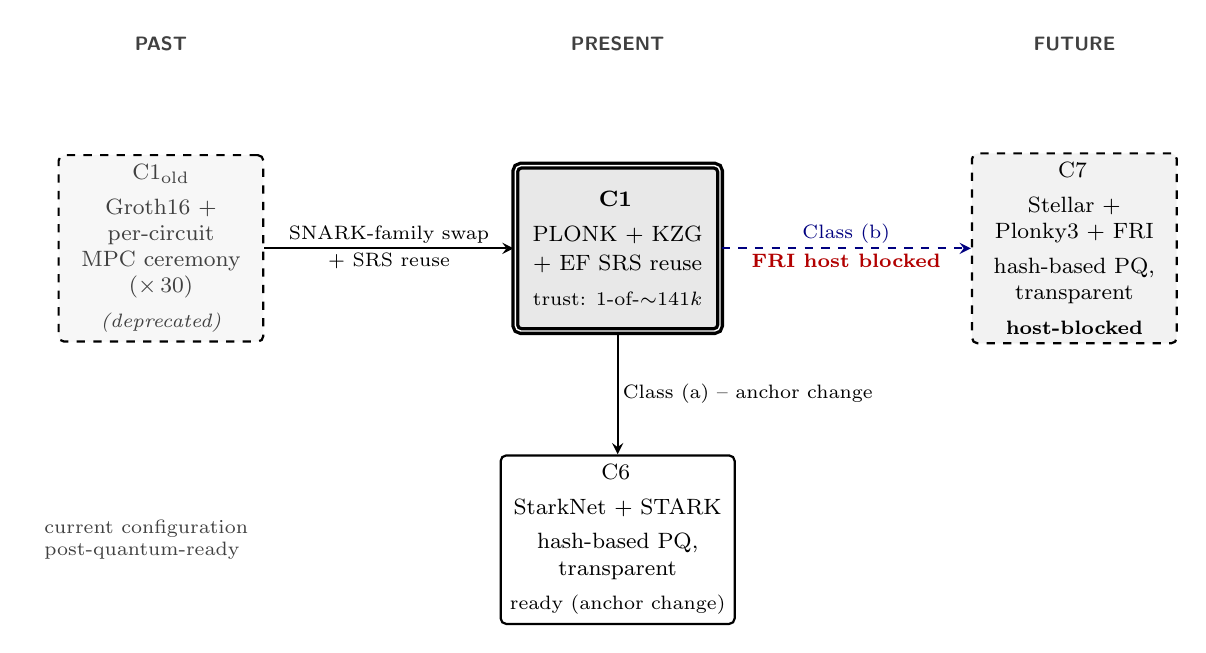
\begin{tikzpicture}[
      nodebase/.style={
        draw, thick, rounded corners=2pt,
        minimum width=2.6cm, minimum height=2.1cm,
        align=center, font=\footnotesize
      },
      deprecated/.style={nodebase, dashed, fill=gray!6,
                         text=gray!50!black},
      current/.style={nodebase, very thick, fill=gray!18,
                      double, double distance=0.5pt},
      pqfuture/.style={nodebase, dashed, fill=gray!10},
      pqalt/.style={nodebase, fill=white},
      arr/.style={->, thick, >=stealth},
      blockedarr/.style={->, thick, dashed, blue!50!black, >=stealth},
      arrlabel/.style={font=\scriptsize, fill=white, inner sep=1.5pt,
                       align=center},
      eralabel/.style={font=\scriptsize\bfseries\sffamily,
                       text=gray!50!black}
    ]
    % Era headers
    \node[eralabel] at ( 0.0, 2.6) {PAST};
    \node[eralabel] at ( 5.8, 2.6) {PRESENT};
    \node[eralabel] at (11.6, 2.6) {FUTURE};

    % Configuration boxes
    \node[deprecated] (old) at ( 0.0, 0) {%
      $\mathrm{C1}_{\mathrm{old}}$\\[3pt]
      Groth16 +\\
      per-circuit\\
      MPC ceremony\\
      ($\times\,30$)\\[3pt]
      \scriptsize\itshape (deprecated)
    };
    \node[current]    (now) at ( 5.8, 0) {%
      \textbf{C1\,$\bigstar$}\\[3pt]
      PLONK + KZG\\[1pt]
      + EF SRS reuse\\[3pt]
      \scriptsize trust: 1-of-${\sim}141\text{k}$
    };
    \node[pqfuture]   (c7)  at (11.6, 0) {%
      $\mathrm{C7}\,\bigstar\bigstar$\\[3pt]
      Stellar +\\
      Plonky3 + FRI\\[3pt]
      hash-based PQ,\\
      transparent\\[3pt]
      \scriptsize\textbf{host-blocked}
    };

    % Off-axis branch: C6
    \node[pqalt]      (c6)  at ( 5.8, -3.7) {%
      $\mathrm{C6}\,\bigstar\bigstar$\\[3pt]
      StarkNet + STARK\\[3pt]
      hash-based PQ,\\
      transparent\\[3pt]
      \scriptsize ready (anchor change)
    };

    % Arrow PAST → PRESENT (nodes placed during the -- operation)
    \draw[arr] (old.east) --
      node[arrlabel, above] {SNARK-family swap}
      node[arrlabel, below] {+ SRS reuse}
      (now.west);

    % Arrow PRESENT → FUTURE (blocked).  Embedded × in label below
    % flags the host-function block.
    \draw[blockedarr] (now.east) --
      node[arrlabel, above] {Class (b)}
      node[arrlabel, below, text=red!70!black]
        {\textbf{FRI host blocked}}
      (c7.west);

    % Branch arrow PRESENT → C6
    \draw[arr] (now.south) --
      node[arrlabel, right] {Class (a) -- anchor change}
      (c6.north);

    % Legend / key
    \node[font=\scriptsize, text=gray!50!black, align=left,
          anchor=west]
      at (-1.7, -3.7)
      {$\bigstar$~current configuration\\
       $\bigstar\bigstar$~post-quantum-ready};
  \end{tikzpicture}}%
  \caption{Trajectory of the C1 deployment through the design
    space. The universal-SRS migration (left arrow) replaced a
    Groth16 + per-circuit-MPC starting point with the analyzed C1
    configuration, collapsing thirty separate trusted-setup
    ceremonies into one SRS reused from the Ethereum Foundation
    KZG ceremony~\cite{eth-kzg-ceremony}. The two PQ-ward
    next-steps available from C1 are the in-place Plonky3 / FRI
    commitment-scheme swap to C7 (host-function-blocked at the
    Stellar verifier layer, Class~(b) of \S\ref{sec:migration})
    and the anchor change to C6 on StarkNet (ready today,
    Class~(a)). Figure~\ref{fig:migration} renders the full
    migration DAG across all surveyed configurations; this
    figure isolates the C1 row.}
  \label{fig:trajectory}
\end{figure}
